\documentclass[a4paper,11pt]{article}

\usepackage[hmargin=2.5cm, vmargin=2cm]{geometry}
\usepackage{paralist}
\usepackage[english,printdayoff]{isodate}
\usepackage[T1]{fontenc}
\usepackage[utf8]{inputenc}
\usepackage[english]{babel}
\usepackage{graphicx}
\usepackage{sectsty}
\usepackage[pdftex,colorlinks=true,urlcolor=blue]{hyperref}

\allsectionsfont{\raggedright}

\newcommand{\myemail}{andrey@rjeutski.com}
\newcommand{\minsk}{Minsk, Belarus}
\newcommand{\periodinminsk}[1]{{\footnotesize #1 in \minsk}}
\newcommand{\jobattributes}[1]{\periodinminsk{#1}{\footnotesize \newline Software Developer}}

\begin{document}
  \pagenumbering{gobble}
  \begin{minipage}{0.69\textwidth}
    \begin{centering}
      {\Huge Andrey Rjeutski}

      Born 1989-04-08 in \minsk\\
      \href{mailto:\myemail}{\myemail} | +49 1575 7742255\\
      Occamstr. 21, 80802 Munich, Germany
      
    \end{centering}
  \end{minipage}
  \begin{minipage}{0.3\textwidth}
    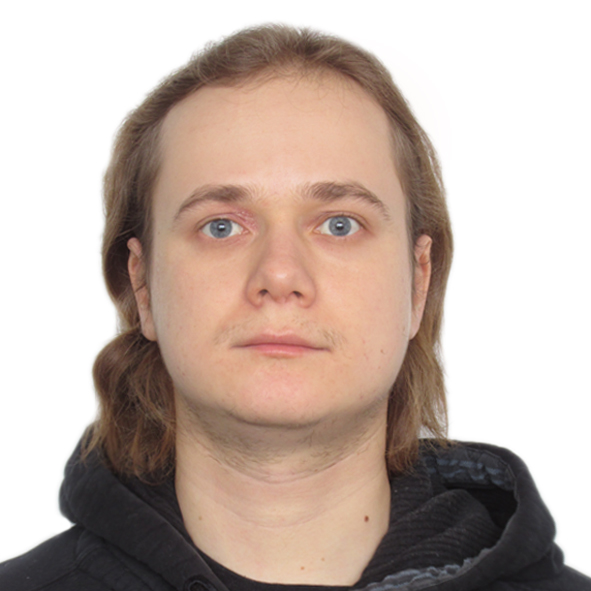
\includegraphics[width=0.95\textwidth]{photo}
  \end{minipage}
  
  \vspace{0.5cm}
  \begin{minipage}[t]{0.34\textwidth}
    \section*{Education} 
    \subsection*{Belarusian State University}
    Faculty of Applied Math and Computer Science\\
    \periodinminsk{2007 to 2012}
    \section*{Links} 
    \href{https://linkedin.com/in/andrey-rjeutski-92064741}{https://linkedin.com/in/andrey-rjeutski-92064741}\\
    \href{https://stackoverflow.com/users/3506292/filhit}{https://stackoverflow.com/\allowbreak users/3506292/filhit}
    \section*{Skills}
    \subsection*{Languages}
    Proficient in english.\\
    Native russian speaker.
    \subsection*{Programming}
    \subsubsection*{Major skills}
    \begin{inparaitem}
      \item C\# 
      \item WPF
      \item ASP .NET MVC
      \item OpenXML
      \item Git
    \end{inparaitem}
    \subsubsection*{Familiar}
    \begin{inparaitem}
      \item ADO .NET 
      \item Linq to SQL
      \item Entity Framework
      \item MSSQL
      \item CruiseControl.Net
      \item SVN
      \item TFVC
      \item Perforce
      \item HTML/CSS
      \item JavaScript
      \item Java
      \item C++
      \item Delphi
    \end{inparaitem}
  \end{minipage}
  \hfill
  \begin{minipage}[t]{0.55\textwidth}
    \section*{Experience}
    \subsection*{\href{http://www.issoft.by/}{ISsoft}}
    \subsubsection*{Microsoft Word add-ins for legal and life sciences industries}
    \jobattributes{\daterange{2013-02-01}{2015-05-01}}
    \begin{itemize}
      \item Implemented the test harness. Time to stabilize a release was reduced from six to two weeks.
      \item Changed the application to be fast and modern looking. A survey has shown that the most of the customers liked the new look and feel.
    \end{itemize}
    \subsubsection*{Desktop application for interest calculation}
    \jobattributes{\daterange{2012-10-01}{2013-01-01}}
    \begin{itemize}
      \item Designed an algorithm to calculate values that were missing in the data exported from the old system. The old system was successfully replaced on time.
    \end{itemize}
    \subsubsection*{SaaS solution for backup in the cloud}
    \jobattributes{\daterange{2012-01-01}{2012-10-01}}
    \begin{itemize}
      \item Developed a SaaS solution to manage and monitor backups online.
    \end{itemize}
    \subsection*{\href{http://www.itransition.com/}{Itransition}}
    \subsubsection*{Online reporting systems for internal corporate usage by pharmaceuticals companies}
    \jobattributes{\daterange{2010-11-01}{2011-12-01}}
    \begin{itemize}
      \item Created a system to present data in charts and tables. Reports were available online and as PDF, PowerPoint and Excel documents.
    \end{itemize}
  \end{minipage}
\end{document}